% p20-f-g-completes-the-following-diagram.tex
%
% Source:   Carl A. Gunter and Dana S. Scott, "Semantic Domains".
%           ScottDomains/papers/Gunter Scott 1990.pdf
% Physical page: 20          Printed page: 19
% Section:  4.4 Sums and lifts.
% Unnamed in the paper (no figure number). Introduced by:
%   "Moreover, if f : D o-> F and g : E o-> F are strict continuous functions,
%    then there is a unique strict continuous function [f, g] which completes
%    the following diagram:"
%
% Content: the universal property of the coalesced sum. Vertices 4, arrows 5
% (4 solid, 1 dashed). Note the arrow directions: inl points DOWN from D into
% D (+) E, inr points UP from E into D (+) E, so both coprojections point at
% the sum; [f, g] is the dashed map out of it.
%
% Geometry measured from a 300 dpi render of the region and divided by
% 118.11 px/cm.
%
\documentclass[border=6pt]{standalone}
\usepackage{tikz}
\begin{document}
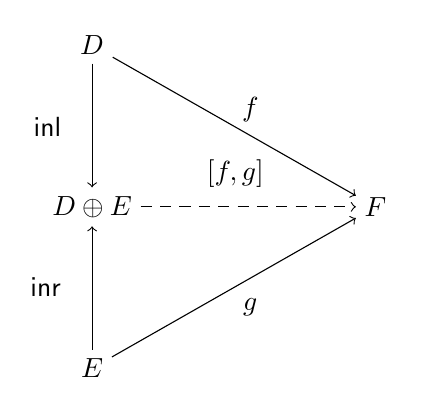
\begin{tikzpicture}[
  x=1cm, y=1cm,
  every node/.style={inner sep=1pt},
  open/.style={circle, draw, fill=white, minimum size=4pt, inner sep=0pt},
  solid/.style={circle, draw, fill=black, minimum size=5pt, inner sep=0pt},
  edge/.style={draw, line width=0.4pt},
  % added for the commutative diagrams: object nodes, and the paper's two
  % arrow kinds -- solid for a named map, dashed for the unique completing map
  obj/.style={inner sep=3pt},
  arrow/.style={draw, line width=0.4pt, ->},
  darrow/.style={draw, line width=0.4pt, ->, dash pattern=on 4pt off 3pt}]

  % vertices
  \node[obj] (d)   at (0.00, 2.05) {$D$};
  \node[obj] (sum) at (0.00, 0.00) {$D \oplus E$};
  \node[obj] (e)   at (0.00,-2.05) {$E$};
  \node[obj] (f)   at (3.60, 0.00) {$F$};

  % arrows
  \draw[arrow]  (d)   -- (sum);
  \draw[arrow]  (e)   -- (sum);
  \draw[arrow]  (d)   -- (f);
  \draw[arrow]  (e)   -- (f);
  \draw[darrow] (sum) -- (f);

  % labels printed inside the picture
  \node[anchor=east]  at (-0.35, 1.02) {\textsf{inl}};
  \node[anchor=east]  at (-0.35,-1.02) {\textsf{inr}};
  \node                at (2.01, 1.23) {$f$};
  \node                at (2.01,-1.27) {$g$};
  \node[anchor=south] at (1.82, 0.20) {$[f,g]$};
\end{tikzpicture}
\end{document}
